\section{Results}
\label{sec:results}

\subsection{Model Evaluation and Validation}
- TODO\\


The advantage of implementing the front end solution, is that changing paramaters as Company, Method and Period is easier. This way, comparing the results achieved with other companies and
methods is fast. 
PipeLine + SVR\\
Tested with different companies - great results\\
Always compared to the benchmark\\


\subsection{Justification}
- TODO\\


- Plot of the predction + data\\

\begin{figure}[H]
\centering
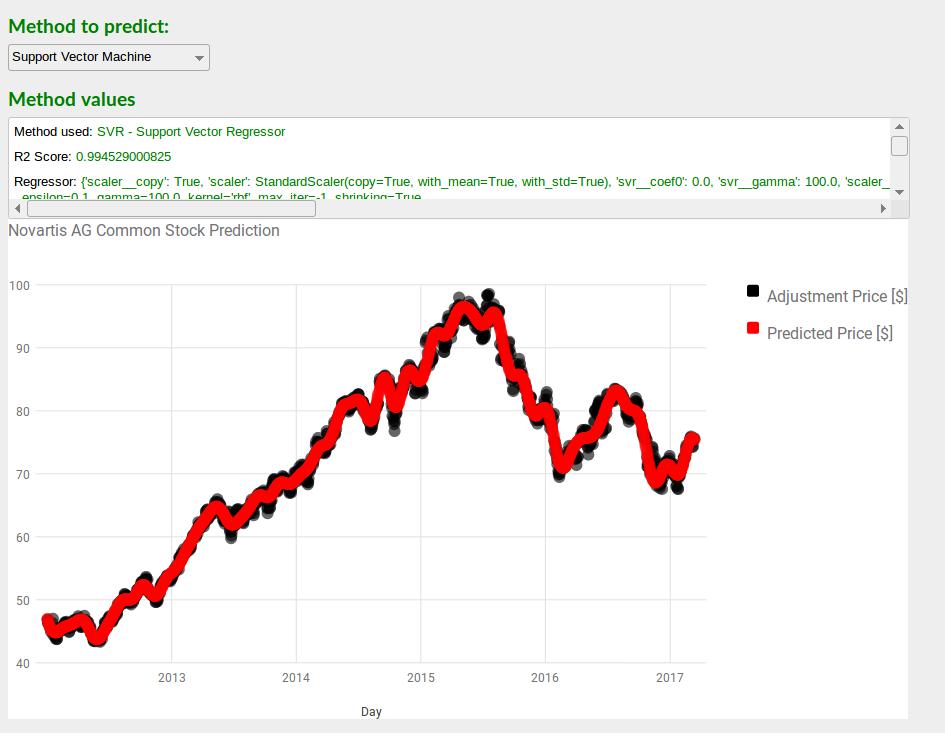
\includegraphics[width=0.6\textwidth]{figures/predict_svr.png}
\caption{NVS: Prediction Results and Historical Data}
\label{fig:predict_svr}
\end{figure}
\ \\
\begin{figure}[H]
\centering
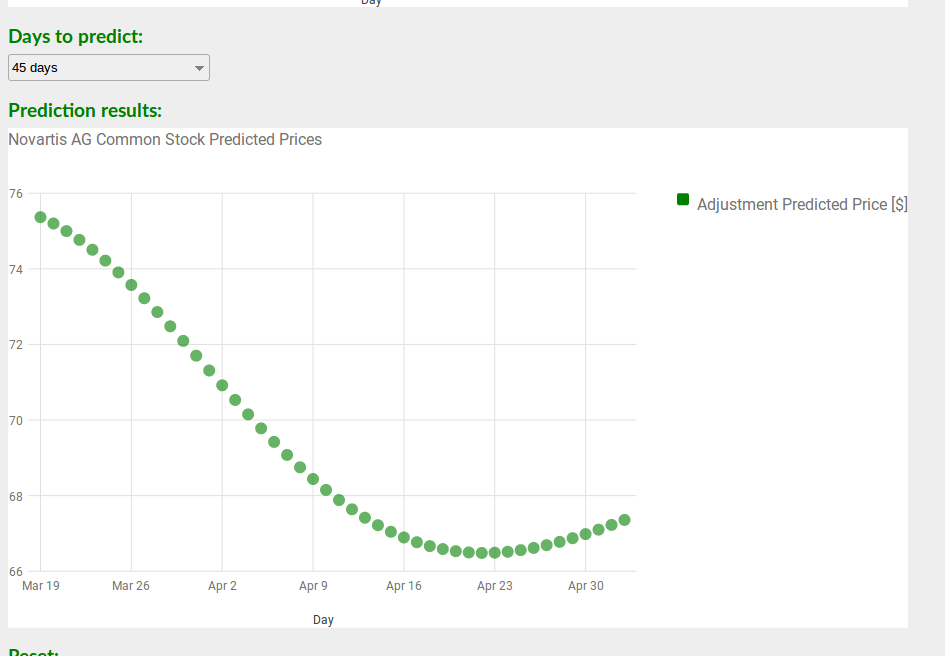
\includegraphics[width=0.6\textwidth]{figures/predict_45days.png}
\caption{NVS: Prediction Results fo 45 days}
\label{fig:predict_45days}
\end{figure}
\ \\

- Strong benchmark\\
- It can be trusted in a shor period (the sentiment of the market is not considered here)\\